\documentclass[a4paper,12pt]{article}
\usepackage[francais]{babel}
\usepackage{array}
\usepackage[utf8]{inputenc}
\usepackage[T1]{fontenc}
\usepackage{amssymb}
\usepackage{colortbl}
\usepackage{graphicx}
\usepackage{hyperref}
\usepackage{fancyhdr}
\usepackage{multicol}
\usepackage{makeidx}

\makeindex
\newcommand{\ndpartie}[0]{La partie s'arrête lorsque l'un des joueurs a gagné, ou lorsque la grille est complétée.}
\newcommand{\athrs}[0]{\bsc{Bordet} Dennis et \bsc{Béziers la Fosse} Thibault}
\title{Tic Tac Toe Evolution}
\author{\athrs}

\pagestyle{fancy}


\begin{document}
\maketitle
\begin{center}
	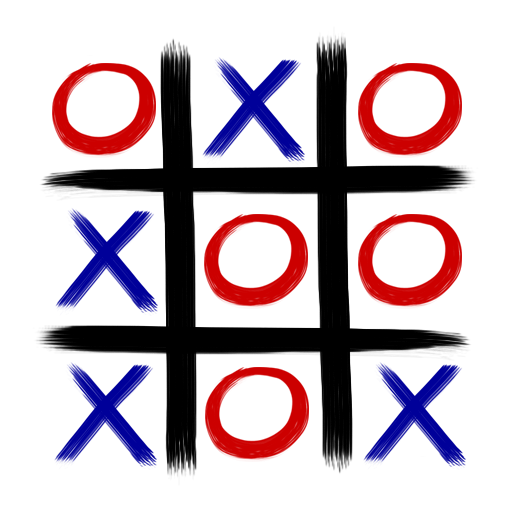
\includegraphics[scale=0.5]{tictactoe.png}
\end {center}

\clearpage
\tableofcontents
\listoffigures

\section{Remerciements}
\phantomsection
Pour ce projet de jeu de Tic-tac-toe nous tenons à remercier nos enseignents de Master ALMA, ainsi que les nombreux étudiants qui ont su nous aider lorsque nous en avions le plus besoin. 
Nous tenons aussi à remercier tout particulièrement nos mamans respectives et la machine à café de l'UFR Sciences et Techniques qui à toujours été là pour nous donner le coup de fouet dont nous avions besoin.
\section{Introduction}
\subsection{Présentation des développeurs}
Nous sommes deux étudiants passionnés d'informatique et de développement d'application logicielle. Nos noms respectifs sont \athrs, et dans le but final de devenir des ingénieurs en informatique aguerris, nous suivons actuellement un Master en Architecture Logicielle. 
Ce jeu est notre 2\up{nd} projet ambitieux de l'année. Nous espérons qu'il vous plaira\ldots
\subsection{Présentation du projet}
Dans le cadre de nos études en architecture logicielle nous avons eu pour projet de concevoir un jeu de tic tac toe dans le langage de notre choix. Nous avons choisis de le développer en \textit{C++}. Effectivement nous manipulons ce langage depuis plusieurs années déjà et pourtant nous apprenons toujours des subtilités à chaque utilisation. C'est donc dans l'optique d'un approfondissement de nos connaissances que nous avons désiré créer ce jeu de la sorte.
\subsection{Présentation du jeu}
Le tic-tac-toe est un jeu de réflexion se pratiquant à deux joueurs au tour par tour et dont le but est de créer le premier un alignement.
 

\section{Installation}
\subsection{Configuration requise}
Pour installer et exécuter le jeu vous devez avoir la configuration suivante: 
\begin{tabular}{|c|r|r|}
	\hline
	\multicolumn{3}{|c|}{\textbf {Configurations requises}} \\
	\hline
	& Configuration Minimale & Configuration Recommandée \\
	\hline
	Processeur & Core i3 @ 1.8GHz & Core i7 @ 3.5GHz  \\
	\hline
	Systeme d'exploitation & Unix 32Bits & Unix 64Bits \\
	\hline
	RAM & 2GB & 4GB \\
	\hline
	Carte Graphique & Radeon 7800 2GB & Radeon 7980 3GB \\
	\hline
\end{tabular}

\subsection{\index{Installation}Installation}
Pour installer le jeu vous devez vous rendre dans le repertoire courant et taper la commande suivante:
\begin{verbatim}
	% make
	% make install 
\end{verbatim}

\subsection{Execution}
Pour lancer le jeu, entrez simplement la commande suivante dans votre terminal Linux:
\verb+tictactoe+

\section{\index{Règles du jeu}Règles du jeu}
Le tic-tac-toe, souvent appelé "Morpion" se joue sur une grille carrée de 3x3 cases. Deux joueurs s'affrontent. Ils doivent remplir chacun à leur tour une case de la grille avec le symbole qui leur est attribué : O ou X. Le gagnant est celui qui arrive à aligner trois symboles identiques, horizontalement, verticalement ou en diagonale.~\cite{wiki}
En raison du nombre de combinaisons limité, l'analyse complète du jeu est facile à réaliser : si les deux joueurs jouent chacun de manière optimale, la partie doit toujours se terminer par un match nul.
Voici un exemple de partie gagnée par le joueur jouant les "X":~
\begin{figure}[h]
	
\includegraphics[scale=0.8]{1.png}
	\caption{Partie gagnée}
	\label{fig:partieGagnee}
\end{figure}

Et un exemple de partie terminée par une égalité:~
\begin{figure}[h]
	
\includegraphics[scale=0.65]{2.png}
	\caption{\'Egalité}
	\label{fig:egalite}
\end{figure}
\section{Fonctionnement du logiciel}
\subsection{Lancement du jeu}~
Une fois le jeu lancé, vous arriverez sur le menu principal après l'affichage des sponsors et de la cinématique de lancement.~ 
Vous aurez le choix entre 5 modes différents:~\begin{itemize}
\item Solo
\item Multijoueur local
\item Multijoueur en ligne
\item Configuration
\item Crédits
\end{itemize}
Choisissez celui de votre choix avec les flèches directionnelles, et validez en appuyant sur Entrée.
\subsection{\index{Comment jouer ?}Comment jouer ?}
Pour jouer à Tic tac toe Ultimate, rien de plus simple ! Sur le côté droit un petit indicateur clignote lorsque que c'est votre tour. Si c'est le cas, vous n'avez qu'à cliquer sur la case de la grille sur laquelle vous désirez poser votre pion. 
\ndpartie 
\subsection{Mode solitaire}
En démarrant le mode solitaire, une nouvelle fenêtre s'ouvrira vous proposant un niveau de difficulté entre 1 et 5:
\begin{enumerate}
\item Novice
\item Amateur
\item Normal
\item Expert
\item Champion
\end{enumerate}
Choisissez donc celui qui vous correspond, et la partie débutera. 
\subsection{Mode multijoueur local}
Le multijoueur local de Tic tac toe ultimate se joue sur un seul ordinateur, au tour par tour. Arrangez vous avec votre ami pour savoir lequel commence, et chacun votre tour cliquez sur la case que vous désirez marquer. 
\ndpartie 
\subsection{\index{Mode online}Mode Multijoueur en réseau}
Pour jouer en ligne, commencez par choisir si vous voulez héberger une partie ou bien rejoindre celle de quelqu'un d'autre. 

\begin{center}
\begin{tabular}{p{6cm}p{6cm}}
	\rowcolor{cyan} Héberger & Rejoindre \\
	Cliquez sur héberger, et donnez l'adresse IP affichée à vos amis, vous devez avoir le port 5555 ouvert & Entrez l'adresse IP à rejoindre et validez.
\end{tabular}
\end{center}

\printindex
\bibliographystyle{plain}
\bibliography{biblio}

\end{document}



